\section{Details of Architecture}
\label{appendix:sec:details_architecture}





\begin{figure*}[t]
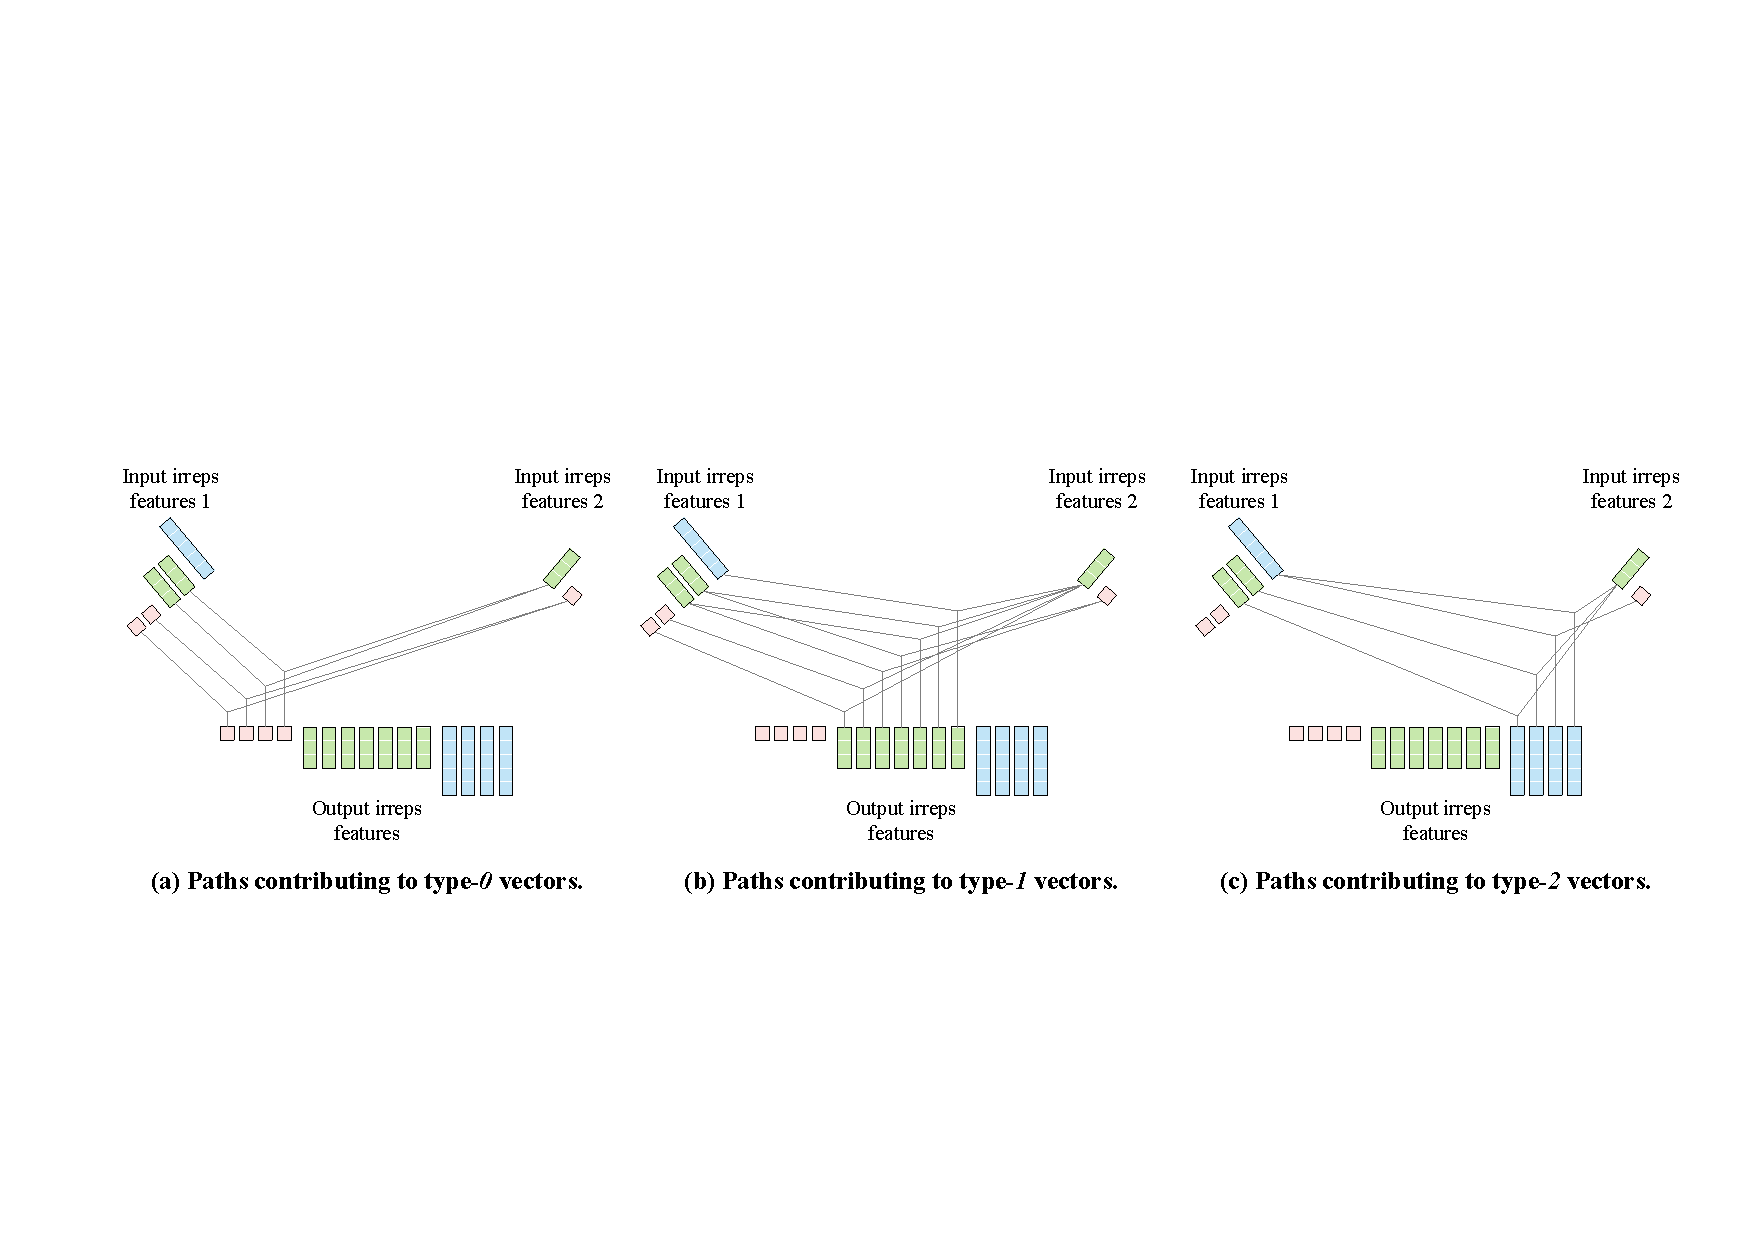
\includegraphics[width=0.99\linewidth]{figure/depthwise_tensor_product_e3nn.pdf}
\centering
\caption{\textbf{An alternative visualization of the depth-wise tensor product. }
We follow the visualization of tensor products in \texttt{e3nn}~\citep{e3nn} and separate paths into three parts based on the types of output vectors.
We note that one vector in the output irreps feature depends only on one vector in each input irreps feature.
}
\label{fig:depthwise_tensor_product_e3nn}
\end{figure*}



\begin{figure*}[th]
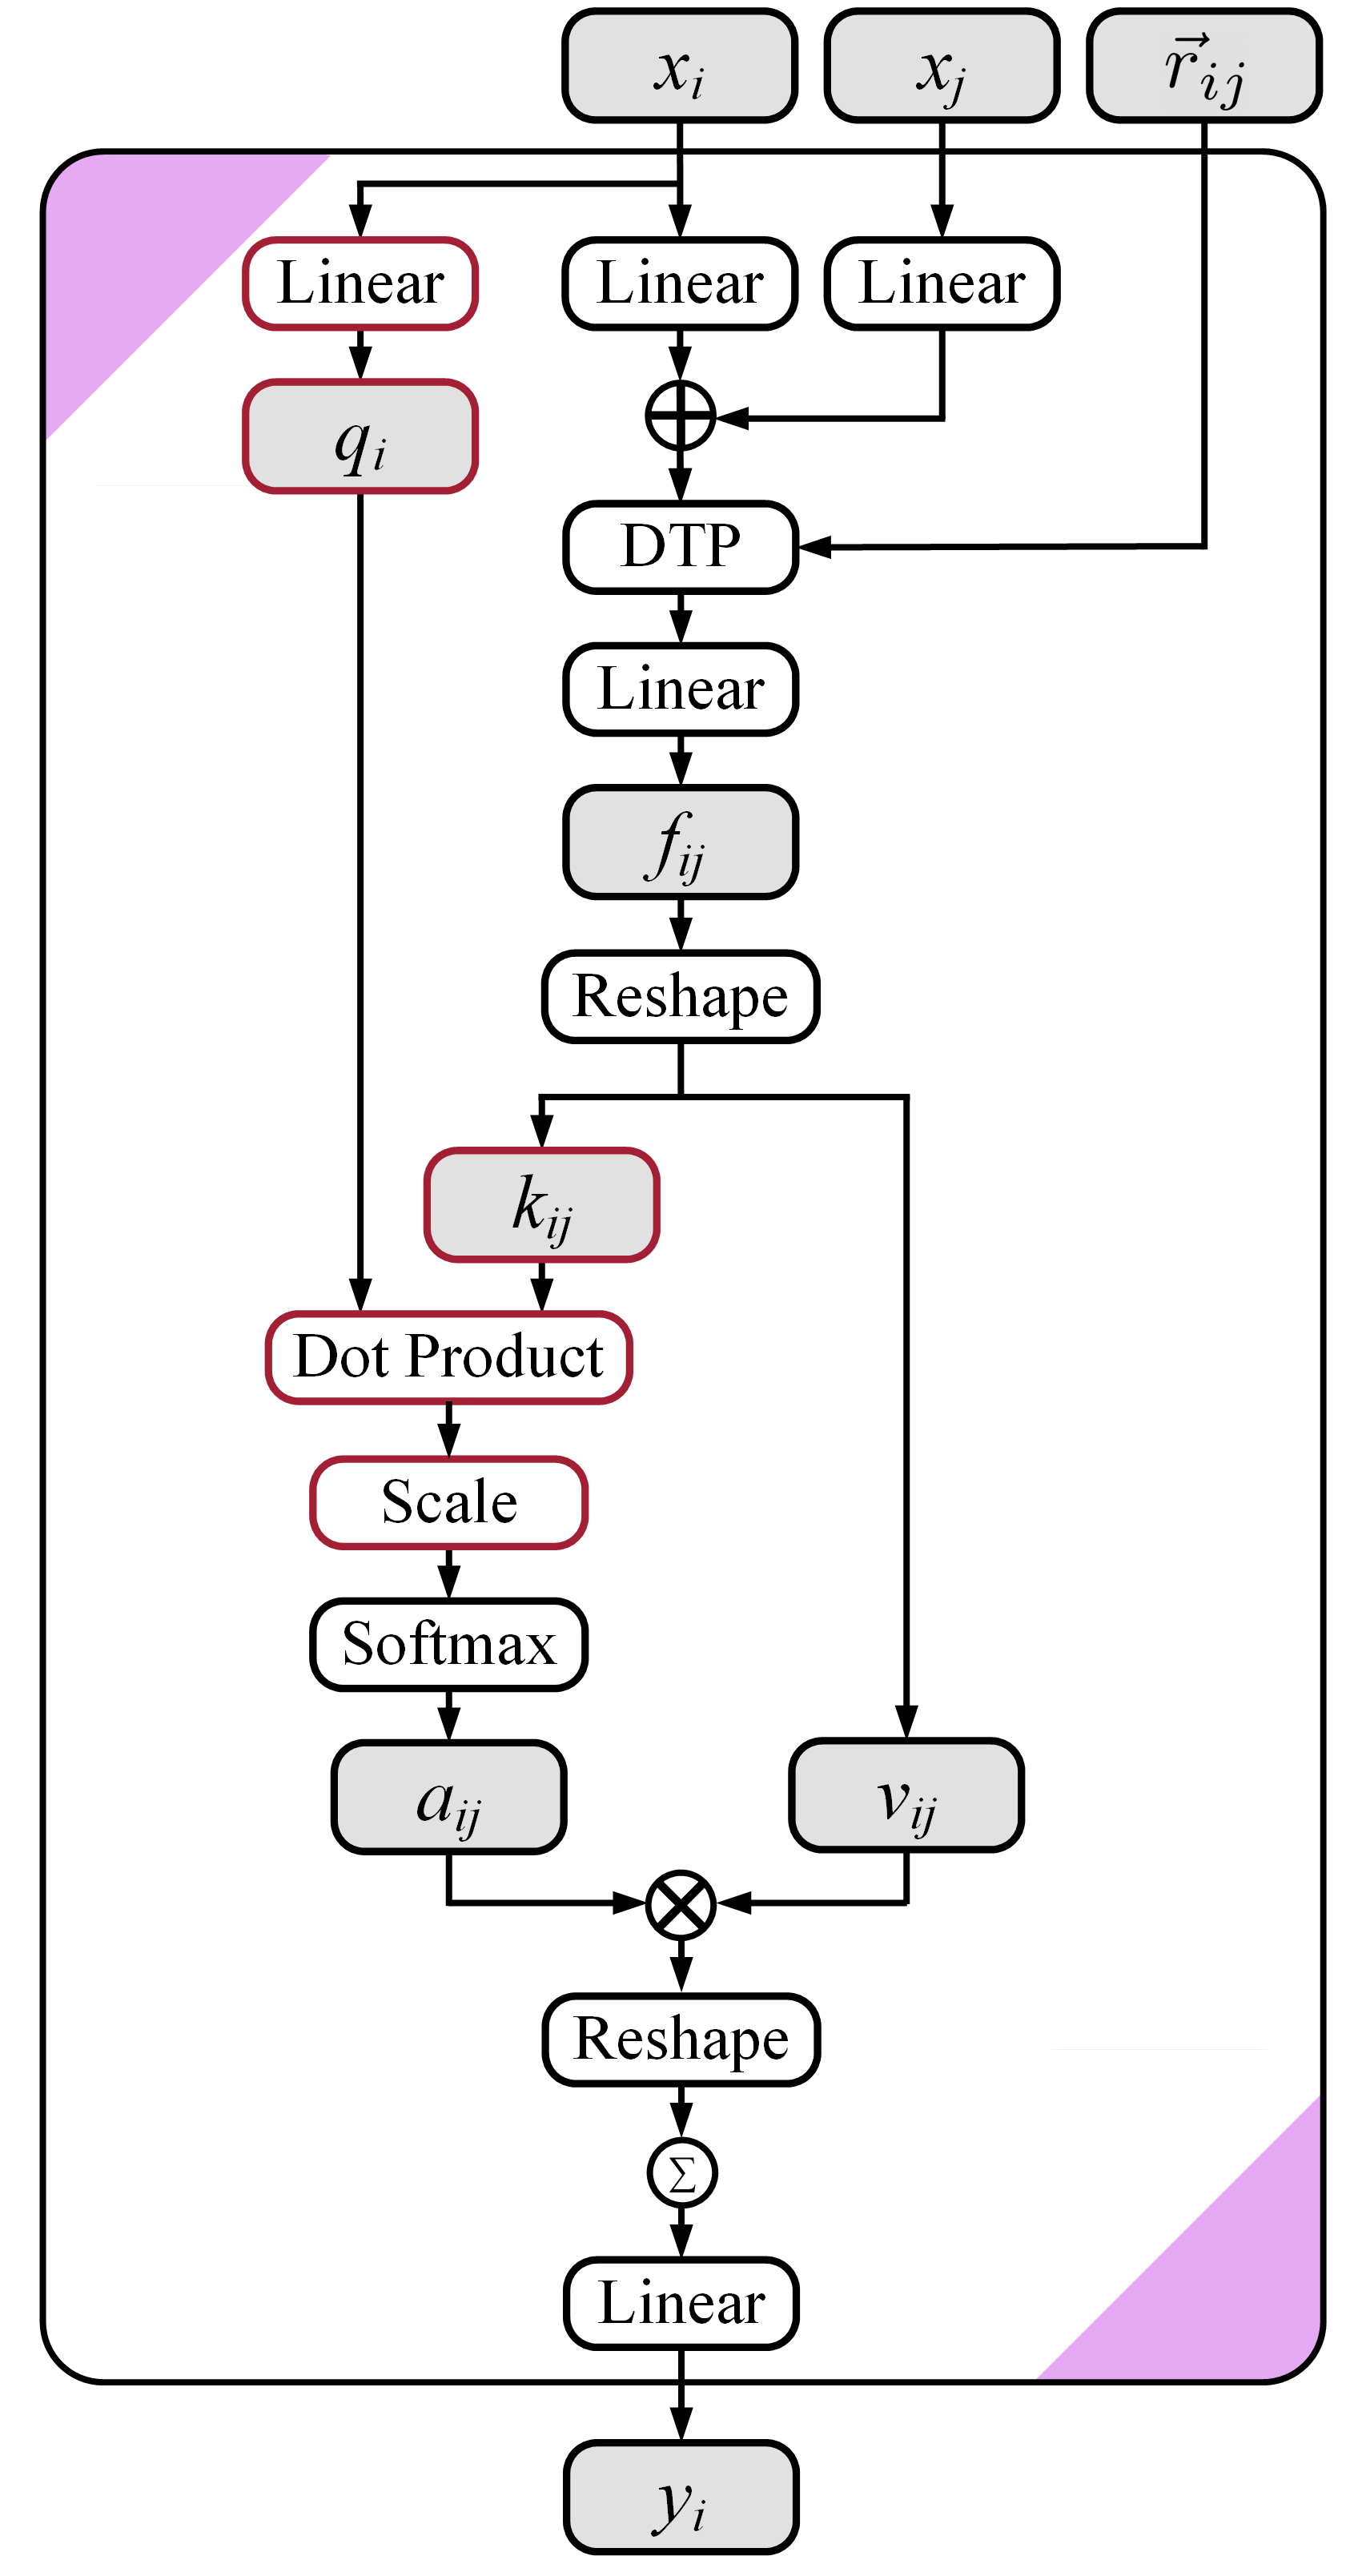
\includegraphics[width=0.35\linewidth]{figure/dot_product_attention.png}
\centering
\caption{\textbf{Architecture of equivariant dot product attention without non-linear message passing.}
In this figure, ``$\otimes$'' denotes multiplication, ``$\oplus$'' denotes addition, and ``DTP'' stands for depth-wise tensor product. $\sum$ within a circle denotes summation over all neighbors.
Gray cells indicate intermediate irreps features.
We highlight the difference of dot product attention from multi-layer perceptron attention in \note{red}.
Note that key $k_{ij}$ and value $v_{ij}$ are irreps features and therefore $f_{ij}$ in dot product attention typically has more channels than that in multi-layer perceptron attention.
}
\label{appendix:fig:dot_product_attention}
\end{figure*}



\subsection{Equivariant Operation Used in Equiformer}
\label{appendix:subsec:equivariant_operations}
We illustrate the equivariant operations used in Equiformer in Fig.~\ref{fig:equivariant_operation} and provide an alternative visualization of depth-wise tensor products in Fig.~\ref{fig:depthwise_tensor_product_e3nn}.

\revision{Besides, we analyze how each equivariant operation remains equivariant and satisfies that $f(D_X(g) x) = D_Y(g) f(x)$, where $f$ is a function mapping between vector spaces $X$ and $Y$, and $D_X(g)$ and $D_Y(g)$ are transformation matrices parametrized by $g$ in $X$ and $Y$.}
\revision{
\begin{enumerate}
    \item \textbf{Linear.} Since for each degree $L$, one output type-$L$ vector is a linear combination of other input type-$L$ vectors, which are transformed by the same matrix $D_X(g)$, the output type-$L$ vector is transformed by the same matrix, meaning that $D_X(g) = D_Y(g)$. 
    \item \textbf{Layer normalization.} For scalar parts ($L = 0$), they are always the same regardless of $E(3)$ transformations, and thus we can apply any function to them. For non-scalar parts ($L > 0$), the L2-norm of any type-$L$ vector is invariant to $E(3)$ transformations. Therefore, the scaling of dividing by the root mean square value (RMS) of L2-norm and multiplying by a learnable parameter $\gamma$ remains the same under $E(3)$ transformations. Multiplying an equivariant feature with an invariant number results in an equivariant feature, and therefore the operation is equivariant. 
    \item \textbf{Gate.} Similar to layer normalization, we can apply any function to the scalar part ($L = 0$). We apply SiLU to the first $C_0$ channels of the scalar part and sigmoid to other channels to obtain non-linear weights. For the non-scalar part ($L > 0$), we multiply each type-$L$ vector with its corresponding non-linear weight. Since the non-linear weights are invariant, multiplying equivariant features with those non-linear weights results in equivariant features.
    \item \textbf{Depth-wise tensor product.} This operation is based on equivariant tensor product operations and restricts that one channel in output irreps feature depends on one channel in input irreps features. The one-to-one dependence of channels does not change the interaction of different type-$L$ vectors, and therefore, the operation is equivariant.
\end{enumerate}
}


\subsection{Equiformer Architecture}
\label{appendix:subsec:equiformer_architecture}

%\todo{Spherical harmonics embeddings}

%\revision{For efficiency and because most works we compare with do not include equivariance to inversion, we mainly adopt $SE(3)$-equivariant irreps features in Equiformer for experiments and note that we can easily incorporate $E(3)$-equivariant irreps features.}
For simplicity and because most works we compare with do not include equivariance to inversion, we adopt $SE(3)$-equivariant irreps features in Equiformer for experiments in the main text and note that $E(3)$-equivariant irreps features can be easily incorporated into Equiformer.
%For clarity, we denote Equiformer with $SE(3)$-equivariant features as ``Equiformer'' and Equiformer with $E(3)$-equivariant features as ``$E(3)$-Equiformer''.

We define architectural hyper-parameters like the number of channels in some layers in Equiformer, which are used to specify the detailed architectures in Sec.~\ref{appendix:subsec:qm9_training_details}, Sec.~\ref{appendix:subsec:md17_training_details} and Sec.~\ref{appendix:subsec:oc20_training_details}.

We use $d_{embed}$ to denote embedding dimension, which defines the dimension of most irreps features.
%Specifically, all irreps features $x_i, y_i$ in Fig.~\ref{fig:equiformer} have dimension $d_{embed}$ unless otherwise stated.
Specifically, all irreps features $x_i, y_i$ in Fig.~\ref{fig:equiformer} have dimension $d_{embed}$ unless otherwise stated.
Besides, we use $d_{sh}$ to represent the dimension of spherical harmonics embeddings of relative positions in all depth-wise tensor products.

%For equivariant graph attention in Fig.~\ref{fig:equiformer}(b), the first two linear layers have the same output dimension $d_{embed}$.
For equivariant graph attention in Fig.~\ref{fig:equiformer}(b), the first two linear layers have the same output dimension $d_{embed}$.
The output dimension of depth-wise tensor products (DTP) are determined by that of input irreps features.
Equivariant graph attention consists of $h$ parallel attention functions, and the value vector in each attention function has dimension $d_{head}$.
We refer to $h$ and $d_{head}$ as the number of heads and head dimension, respectively.
By default, we set the number of channels in scalar feature $f_{ij}^{(0)}$ to be the same as the number of channels of type-$0$ or type-$(0, e)$ vectors in $v_{ij}$.
When non-linear messages are adopted in $v_{ij}$, we set the dimension of output irreps features in gate activation to be $h \times d_{head}$.
Therefore, we can use two hyper-parameters $h$ and $d_{head}$ to specify the detailed architecture of equivariant graph attention.

As for feed forward networks (FFNs), we denote the dimension of output irreps features in gate activation as $d_{ffn}$.
The FFN in the last Transformer block has output dimension $d_{feature}$, and we set $d_{ffn}$ of the last FFN, which is followed by output head, to be $d_{feature}$ as well.
Thus, two hyper-parameters $d_{ffn}$ and $d_{feature}$ are used to specify architectures of FFNs and the output dimension after Transformer blocks.

Irreps features contain channels of vectors with degrees up to $L_{max}$.
We denote $C_L$ type-$L$ vectors as $(C_L, L)$ and $C_{(L, p)}$ type-$(L, p)$ vectors as $(C_{(L, p)}, L, p)$ and use brackets to represent concatenations of vectors.
For example, the dimension of irreps features containing $256$ type-$0$ vectors and $128$ type-$1$ vectors can be represented as $[(256, 0), (128, 1)]$.
%We can extend this to include inversion by introducing parity $p$ and using $(C_{(L, p)}, L, p)$.







\subsection{Dot Product Attention}
\label{appendix:subsec:dot_product_attention}
%We illustrate the dot product attention without non-linear message passing used in ablation study in Fig.~\ref{fig:dot_product_attention}.
We illustrate the dot product attention without non-linear message passing used in ablation study in Fig.~\ref{appendix:fig:dot_product_attention}.
The architecture is adapted from SE(3)-Transformer~\citep{se3_transformer}.
The difference from multi-layer perceptron attention lies in how we obtain attention weights $a_{ij}$ from $f_{ij}$.
We split $f_{ij}$ into two irreps features, key $k_{ij}$ and value $v_{ij}$, and obtain query $q_{i}$ with a linear layer.
Then, we perform scaled dot product~\citep{transformer} between $q_i$ and $k_{ij}$ for attention weights.


\subsection{\revision{Incorporating $E(3)$-Equivariance}}
\label{appendix:subsec:incorporating_e3_equivariance}
\revision{To incorporate $E(3)$-equivariance to Equiformer, we can directly use the same architecture described in Fig.~\ref{fig:equiformer} with the following two modifications:}
\revision{
\begin{enumerate}
    \item We change internal representations from type-$L$ vectors to type-$(L, p)$ vectors as mentioned in Sec.~\ref{appendix:subsec:equivariant_irreps_feature}. Note that type-$(L, e)$ vectors and type-$(L, o)$ vectors are considered different types by equivariant operations and that scalars correspond to only type-$(0, e)$ vectors and do not include type-$(0, o)$ vectors. 
    \item The behaviors of equivariant operations are changed accordingly since parities $p$ are included in internal representations. 
    The operations of linear and layer normalization will treat type-$(L, e)$ vectors and type-$(L, o)$ vectors as different types. 
    This means that we linearly combine or normalize these two types of vectors in a separate manner. 
    In Sec.~\ref{appendix:subsec:tensor_product}, we discuss how tensor products behave when $E(3)$ equivariance is considered. 
    For the operation of gate, we apply activation functions to type-$(0, e)$ vectors (scalars) and treat type-$(0, o)$ vectors (pseudo-scalars) in the same manner as vectors of higher $L$. 
    Specifically, given input $x$ containing non-scalar $C_{(L, p)}$ type-$(L, p)$ vectors with $0 < L \leq L_{max}$ and $p \in \{e, o\}$, $C_{(0, o)}$ type-$(0, o)$ vectors and $(C_{(0, e)} + C_{(0, o)} + \sum_{L=1}^{L_{max}} \sum_{p \in \{e, o\}}C_{(L, p)})$ type-$(0, e)$ vectors, we apply SiLU to the first $C_{(0, e)}$ type-$(0, e)$ vectors and sigmoid function to the other $( C_{(0, o)} + \sum_{L=1}^{L_{max}} \sum_{p \in \{e, o\}}C_{(L, p)})$ type-$(0, e)$ vectors to obtain non-linear weights and multiply each pseudo-scalar or type-$(L, p)$ vector with corresponding non-linear weights. After the gate activation, the number of channels for type-$(0, e)$ vectors is reduced to $C_{(0, e)}$.  
\end{enumerate}
}
\revision{}

\subsection{Discussion on Computational Complexity}
\label{appendix:subsec:computational_complexity}


We discuss the computational complexity of the proposed equivariant graph attention here.

First, we compare dot product attention with MLP attention when linear messages are used for value $v_{ij}$.
Dot product attention requires taking the dot product of two irreps features, query $q_i$ and key $k_{ij}$, for attention weights, and both $q_i$ and $k_{ij}$ have the same dimension as value $v_{ij}$.
In contrast, MLP attention uses only scalar features $f_{ij}^{(0)}$ for attention weights.
The dimension of scalar features $f_{ij}^{(0)}$ is the same as that of the scalar part of $v_{ij}$.
Therefore, MLP attention generates less and smaller intermediate features for attention weights and is faster than dot product attention.

Second, compared to linear messages, using non-linear messages increases the number of tensor product operations from $1$ to $2$.
Since tensor products are compute-intensive, this inevitably increases training and inference time.

Please refer to Sec.~\ref{appendix:subsec:qm9_training_details} and Sec.~\ref{appendix:subsec:oc20_training_details} for the exact numbers of training time on QM9 and OC20.